\documentclass[conference]{IEEEtran}

% ===================== Packages =====================
\usepackage{cite}
\usepackage{amsmath,amssymb,amsfonts}
\usepackage{algorithmic}
\usepackage{graphicx}
\usepackage{textcomp}
\usepackage{xcolor}
\usepackage{hyperref}
\usepackage{booktabs}
\usepackage{multirow}
\usepackage{listings}
\usepackage{tikz}
\usetikzlibrary{shapes.geometric, arrows.meta, positioning, fit, backgrounds}
\usepackage{float}
\usepackage{enumitem}
\usepackage{url}
\usepackage{balance}

% ===================== Hyperref Setup =====================
\hypersetup{
    colorlinks=true,
    linkcolor=blue,
    citecolor=blue,
    urlcolor=blue
}

% ===================== Listings Setup =====================
\lstset{
    basicstyle=\ttfamily\footnotesize,
    backgroundcolor=\color{gray!10},
    frame=single,
    framerule=0.5pt,
    rulecolor=\color{gray!50},
    breaklines=true,
    captionpos=b,
    tabsize=2,
    showstringspaces=false,
    keywordstyle=\color{blue}\bfseries,
    stringstyle=\color{red!70!black},
    commentstyle=\color{green!50!black}\itshape
}

\def\BibTeX{{\rm B\kern-.05em{\sc i\kern-.025em b}\kern-.08em
    T\kern-.1667em\lower.7ex\hbox{E}\kern-.125emX}}

\begin{document}

% ===================== Title =====================
\title{Social Media Sentiment Analysis Using Big Data and Natural Language Processing}

\author{
    \IEEEauthorblockN{Mohammed Badawi}
    \IEEEauthorblockA{
        \textit{Student ID: 2105656} \\
        \textit{Course: Big Data \& Artificial Intelligence} \\
        \textit{Submission: Project Proposal} \\
        \textit{Date: April 17, 2026}
    }
}

\maketitle

% ===================== Abstract =====================
\begin{abstract}
The exponential growth of social media platforms has created an unprecedented volume of user-generated textual data, presenting both challenges and opportunities for large-scale sentiment analysis. This proposal presents the design of a comprehensive Big Data and Artificial Intelligence system for real-time and batch sentiment analysis of social media content sourced from Twitter (X) and Reddit. The proposed architecture leverages Apache Kafka for distributed data ingestion, Apache Spark for scalable batch and streaming processing, MongoDB as a flexible NoSQL data store, and a suite of Natural Language Processing models---including Logistic Regression, Bidirectional LSTM, and fine-tuned BERT---for multi-class sentiment classification. The system follows a Lambda-like architecture to support both real-time inference and periodic batch retraining. Evaluation will encompass both model-level metrics (accuracy, F1-score, ROC-AUC) and system-level performance indicators (throughput, latency, scalability). The project addresses the core Big Data dimensions of volume, velocity, and variety inherent in social media data.
\end{abstract}

\begin{IEEEkeywords}
Sentiment Analysis, Big Data, Natural Language Processing, Apache Spark, Apache Kafka, MongoDB, BERT, Deep Learning, Social Media Analytics
\end{IEEEkeywords}

% ===================== 1. Problem Definition =====================
\section{Problem Definition}

\subsection{Overview}
The rapid growth of social media platforms such as Twitter (X), Reddit, and Facebook has generated an unprecedented volume of user-generated content. Every day, billions of posts, comments, and reactions are published, expressing opinions on topics ranging from politics and public health to product reviews and entertainment~\cite{go2009twitter}. Extracting meaningful insights from this massive stream of unstructured text is both a challenge and an opportunity.

This project proposes a scalable, end-to-end Big Data and AI pipeline for performing sentiment analysis on social media data. The system will ingest raw social media posts in real time, preprocess the text using distributed computing, store results in a NoSQL database, and classify each post as \textit{positive}, \textit{negative}, or \textit{neutral} using state-of-the-art NLP models.

\subsection{Motivation}
Traditional sentiment analysis tools are not designed to operate on the scale demanded by modern social media. A single trending hashtag can produce millions of tweets within hours, far exceeding the processing capacity of conventional, single-node systems~\cite{zaharia2016apache}. There is a clear need for a scalable, distributed solution capable of ingesting, processing, and classifying this data in near-real time. Moreover, the informal and noisy nature of social media text---containing slang, abbreviations, emojis, and code-switching---poses significant challenges for standard NLP pipelines, necessitating robust preprocessing and advanced language models.

\subsection{Real-World Significance}
The proposed system addresses several high-impact real-world applications:
\begin{itemize}[leftmargin=*]
    \item \textbf{Business Intelligence:} Companies can monitor brand perception and react to customer feedback promptly, enabling data-driven marketing strategies.
    \item \textbf{Public Health:} Health authorities can track public sentiment around vaccination campaigns, disease outbreaks, and mental health trends at population scale.
    \item \textbf{Politics \& Policy:} Political analysts can gauge public opinion before and after policy announcements, supporting evidence-based governance.
    \item \textbf{Financial Markets:} Sentiment signals extracted from social data have been shown to correlate with stock price movements and market volatility~\cite{kreps2011kafka}.
    \item \textbf{Crisis Management:} During natural disasters or public emergencies, real-time sentiment monitoring can help coordinate response efforts and identify areas of greatest need.
\end{itemize}

\subsection{Why Big Data and AI?}
The sheer \textit{volume} (hundreds of millions of posts daily), \textit{velocity} (continuous real-time streams), and \textit{variety} (emojis, slang, hashtags, multilingual content) of social media data make it a canonical Big Data problem. A distributed infrastructure is required to ingest and process the data at scale, while advanced Natural Language Processing (NLP) and Machine Learning (ML) models are needed to classify sentiments accurately~\cite{devlin2019bert}. The convergence of these two domains---Big Data infrastructure and AI---is essential to build a system that is both scalable and intelligent.

% ===================== 2. Dataset Description =====================
\section{Dataset Description \& Visualisation}

\subsection{Dataset Selection}
This project will utilise two complementary datasets to ensure diversity and robustness:

\begin{enumerate}[leftmargin=*]
    \item \textbf{Sentiment140 Dataset} -- A widely used benchmark dataset containing 1.6 million tweets labelled as positive, negative, or neutral using distant supervision. Available on Kaggle at: \url{https://www.kaggle.com/datasets/kazanova/sentiment140}~\cite{go2009twitter}.
    \item \textbf{Reddit Comments Dataset} -- Collected via the Reddit Pushshift API, containing posts from subreddits related to technology, news, and consumer products. Approximately 500k--1M comments will be used, providing a complementary source with longer text and community-driven scoring.
\end{enumerate}

\subsection{Dataset Characteristics}

\begin{table}[H]
\centering
\caption{Summary of Dataset Characteristics}
\label{tab:dataset}
\renewcommand{\arraystretch}{1.15}
\begin{tabular}{@{}lcc@{}}
\toprule
\textbf{Attribute} & \textbf{Twitter (Sent140)} & \textbf{Reddit Comments} \\
\midrule
Size & $\sim$1.6M records & $\sim$1M records \\
Format & CSV & JSON (via API) \\
Language & English & English \\
Labels & Pos / Neg / Neutral & Unlabelled \\
Key Features & text, user, time, polarity & body, score, subreddit \\
\bottomrule
\end{tabular}
\end{table}

The combined dataset of approximately 2.6 million records ensures sufficient volume for training deep learning models and stress-testing the distributed pipeline.

\subsection{Exploratory Data Analysis (EDA)}
The following EDA steps will be performed and visualised to understand the data distribution and guide preprocessing decisions:
\begin{itemize}[leftmargin=*]
    \item \textbf{Class Distribution:} Bar charts showing the distribution of positive, negative, and neutral labels to assess class imbalance.
    \item \textbf{Tweet/Post Length:} Histograms of character and word counts to understand text length distribution and inform padding/truncation strategies.
    \item \textbf{Word Clouds:} Separate word clouds for each sentiment class to identify discriminative vocabulary.
    \item \textbf{Temporal Trends:} Line graphs plotting sentiment scores over time to identify seasonal or event-driven patterns.
    \item \textbf{Top Hashtags/Keywords:} Frequency plots of the most common tokens per class to support feature engineering.
    \item \textbf{Correlation Analysis:} Heatmaps showing correlations between metadata features (post length, hashtag count, time of day) and sentiment labels.
\end{itemize}

All visualisations will be generated using \texttt{matplotlib}, \texttt{seaborn}, and \texttt{wordcloud} within a distributed PySpark environment to handle the full dataset scale.

% ===================== 3. Data Preprocessing =====================
\section{Data Preprocessing}

Raw social media text is inherently noisy and requires careful preprocessing to ensure high-quality input for downstream models. The preprocessing pipeline will involve the following stages, implemented as Spark transformations for distributed execution.

\subsection{Text Cleaning}
\begin{itemize}[leftmargin=*]
    \item Remove URLs, HTML tags, and special characters using regular expressions.
    \item Strip usernames (@mentions) and hashtag symbols (retaining the hashtag word for semantic content).
    \item Normalise whitespace and convert text to lowercase.
    \item Handle emojis: convert to text descriptions using the \texttt{emoji} Python library or remove entirely for baseline experiments.
    \item Remove duplicate and near-duplicate posts using MinHash-based deduplication.
\end{itemize}

\subsection{Tokenisation and Normalisation}
\begin{itemize}[leftmargin=*]
    \item Tokenise text using NLTK or SpaCy tokenisers.
    \item Apply lemmatisation to reduce words to their base forms (e.g., ``running'' $\rightarrow$ ``run'').
    \item Remove English stop words using a curated stop word list that preserves negation words (e.g., ``not'', ``never'') critical for sentiment analysis.
\end{itemize}

\subsection{Feature Engineering}
Multiple feature representations will be generated to support different model architectures:
\begin{itemize}[leftmargin=*]
    \item \textbf{TF-IDF Vectors:} Computed using Spark MLlib's \texttt{HashingTF} and \texttt{IDF} transformers for traditional ML models.
    \item \textbf{Word Embeddings:} Pre-trained GloVe (200-dimensional) or Word2Vec embeddings for deep learning models, enabling transfer learning from large corpora.
    \item \textbf{Sentiment Lexicon Features:} VADER sentiment scores appended as additional numerical features to provide lexicon-based signals.
    \item \textbf{Metadata Features:} Post length, number of hashtags, presence of exclamation marks, hour of posting, and platform source indicator.
\end{itemize}

\subsection{Handling Missing Values}
Rows with null or empty text fields will be removed. Posts shorter than 3 tokens after cleaning will be discarded as uninformative. For the Reddit dataset, missing score values will be imputed with the subreddit-level median to preserve the record.

\subsection{Train/Test Split}
An 80/10/10 split (train/validation/test) will be applied, stratified by class label to preserve class distribution across all splits. Temporal ordering will be respected where possible to simulate realistic deployment conditions.

% ===================== 4. NoSQL Database =====================
\section{NoSQL Database}

\subsection{Chosen Database: MongoDB}
MongoDB will be used as the primary NoSQL store for both raw and processed data~\cite{chodorow2013mongodb}. Its document-oriented model is ideal for storing semi-structured social media posts, which vary significantly in schema---some tweets include geo-location data, others contain embedded media URLs, and Reddit posts carry unique metadata such as subreddit names and community scores.

\subsection{Data Modelling Strategy}
Each social media post will be stored as a BSON document with the following schema:

\begin{lstlisting}[language=java, caption={MongoDB Document Schema}]
{
  "_id": ObjectId,
  "source": "twitter" | "reddit",
  "text": "raw post text",
  "clean_text": "preprocessed text",
  "timestamp": ISODate,
  "user_id": string,
  "sentiment": "positive"|"negative"|"neutral",
  "confidence": float,
  "metadata": {
    "hashtags": ["tag1", "tag2"],
    "word_count": int,
    "platform_score": int,
    "processing_time_ms": int
  }
}
\end{lstlisting}

Indexes will be created on \texttt{timestamp}, \texttt{sentiment}, and \texttt{source} fields to support efficient time-range queries and aggregation operations. A TTL (Time-To-Live) index on \texttt{timestamp} will automatically expire old records beyond the retention window.

\subsection{Justification for NoSQL}
\begin{itemize}[leftmargin=*]
    \item \textbf{Schema Flexibility:} Social media posts differ in structure across platforms; NoSQL avoids rigid schema constraints and accommodates evolving data formats.
    \item \textbf{Horizontal Scalability:} MongoDB supports sharding across multiple nodes, handling millions of documents efficiently with automatic data distribution.
    \item \textbf{High Write Throughput:} Critical for real-time ingestion of streaming data, MongoDB's write-ahead logging and memory-mapped storage engine provide excellent write performance.
    \item \textbf{Rich Query Support:} MongoDB's aggregation pipeline enables complex analytical queries---including group-by, time-windowed aggregations, and text search---directly on stored data without requiring a separate analytics layer.
\end{itemize}

% ===================== 5. Big Data Infrastructure =====================
\section{Big Data Infrastructure}

\subsection{Apache Kafka -- Data Ingestion}
Apache Kafka will serve as the distributed message broker, simulating a real-time data stream from the Twitter and Reddit APIs~\cite{kreps2011kafka}. Producers will publish raw posts to dedicated Kafka topics (\texttt{twitter-stream}, \texttt{reddit-stream}), and Spark Structured Streaming will act as the consumer. Kafka's partitioning mechanism ensures horizontal scalability and fault tolerance, with configurable replication factors for data durability.

\subsection{Apache Spark -- Distributed Processing}
Apache Spark will be the core processing engine for both batch preprocessing and real-time streaming inference~\cite{zaharia2016apache}:
\begin{itemize}[leftmargin=*]
    \item \textbf{Spark SQL:} For structured data transformations, schema enforcement, and interactive EDA on large datasets.
    \item \textbf{Spark MLlib:} For training TF-IDF + Logistic Regression and Naive Bayes baseline models in a distributed fashion, leveraging data parallelism.
    \item \textbf{Spark Structured Streaming:} For consuming Kafka topics and running inference in micro-batches with exactly-once processing semantics.
\end{itemize}

\subsection{Distributed Storage}
Processed datasets and model artefacts will be stored in HDFS (Hadoop Distributed File System) in Parquet format for efficient columnar access and compression. MongoDB will serve as the operational store for query-ready records and real-time dashboard queries. The dual-storage strategy separates analytical workloads (HDFS/Parquet) from operational workloads (MongoDB).

\subsection{Pipeline Orchestration}
Apache Airflow will be used to schedule and monitor batch preprocessing and retraining jobs, providing a clear DAG-based (Directed Acyclic Graph) workflow management interface. Airflow DAGs will handle:
\begin{itemize}[leftmargin=*]
    \item Scheduled batch data ingestion from API dumps
    \item Periodic model retraining on accumulated data
    \item Data quality checks and pipeline health monitoring
    \item Alerting on pipeline failures or performance degradation
\end{itemize}

% ===================== 6. AI Application =====================
\section{AI Application}

\subsection{Task}
The core AI task is \textit{multi-class text classification}: classifying each social media post as \textbf{Positive}, \textbf{Negative}, or \textbf{Neutral} based on its textual content and metadata features.

\subsection{Model Selection}
Three models of increasing complexity will be developed and compared to establish a performance-scalability trade-off:

\begin{enumerate}[leftmargin=*]
    \item \textbf{Logistic Regression (Baseline)} -- Trained on TF-IDF features using Spark MLlib. This model is fast, interpretable, and serves as the baseline for comparison. It can be trained distributedly on the full dataset.
    
    \item \textbf{Bidirectional LSTM (Deep Learning)} -- Trained with pre-trained GloVe embeddings (200d) using TensorFlow/Keras. The bidirectional architecture captures both forward and backward sequential context in text, providing richer representations than bag-of-words approaches.
    
    \item \textbf{BERT-based Fine-Tuning (State-of-the-Art)} -- Fine-tuning a pre-trained \texttt{bert-base-uncased} model via HuggingFace Transformers on the labelled dataset~\cite{devlin2019bert}. BERT's contextual embeddings and attention mechanism enable nuanced understanding of sentiment, including sarcasm and negation.
\end{enumerate}

\subsection{Training Process}
\begin{itemize}[leftmargin=*]
    \item The baseline Logistic Regression model will be trained distributedly using Spark MLlib on the full 1.6M tweet dataset, completing in minutes.
    \item LSTM and BERT models will be trained on a GPU-enabled node using PyTorch/TensorFlow, with the dataset stored in HDFS and loaded in batches via custom data loaders.
    \item Hyperparameter tuning will be performed using grid search (for MLlib models) and Optuna (for deep learning models), optimising learning rate, batch size, dropout rate, and number of epochs.
    \item Early stopping with patience of 3 epochs will be applied to prevent overfitting on deep learning models.
\end{itemize}

\subsection{Evaluation}
Models will be evaluated on the held-out test set using the following metrics:
\begin{itemize}[leftmargin=*]
    \item \textbf{Accuracy} -- Overall correct classification rate.
    \item \textbf{Precision, Recall, F1-Score} -- Computed per class and aggregated (macro and weighted averages).
    \item \textbf{Confusion Matrix} -- Visual analysis of misclassification patterns.
    \item \textbf{ROC-AUC} -- One-vs-rest area under the ROC curve for multi-class discrimination.
\end{itemize}

% ===================== 7. System Architecture =====================
\section{System Architecture}

\subsection{Architecture Overview}
The system follows a \textit{Lambda-like architecture} with both a real-time streaming layer and a batch processing layer, unified through a common serving layer backed by MongoDB. This hybrid approach ensures low-latency predictions for incoming data while enabling periodic model retraining on accumulated historical data.

\subsection{Architecture Diagram}

\begin{figure}[H]
\centering
\resizebox{\columnwidth}{!}{%
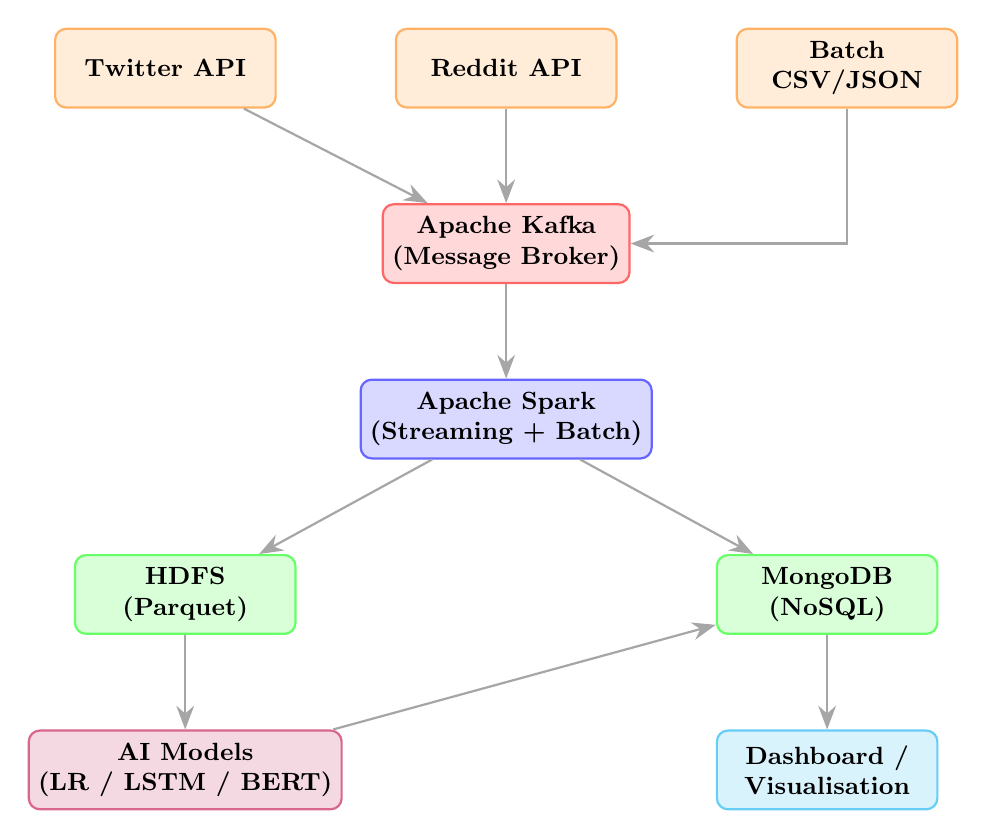
\begin{tikzpicture}[
    node distance=1.2cm and 1.5cm,
    box/.style={draw, rounded corners, minimum height=1cm, minimum width=2.8cm, 
                align=center, font=\small\bfseries, fill=#1!15, draw=#1!60, line width=0.8pt},
    box/.default=blue,
    arrow/.style={-{Stealth[length=3mm]}, thick, color=gray!70},
    label/.style={font=\tiny\itshape, text=gray}
]

% Data Sources
\node[box=orange] (twitter) {Twitter API};
\node[box=orange, right=1.5cm of twitter] (reddit) {Reddit API};
\node[box=orange, right=1.5cm of reddit] (batch) {Batch\\CSV/JSON};

% Kafka
\node[box=red, below=1.2cm of reddit] (kafka) {Apache Kafka\\(Message Broker)};

% Spark
\node[box=blue, below=1.2cm of kafka] (spark) {Apache Spark\\(Streaming + Batch)};

% Storage
\node[box=green, below left=1.2cm and 0.8cm of spark] (hdfs) {HDFS\\(Parquet)};
\node[box=green, below right=1.2cm and 0.8cm of spark] (mongo) {MongoDB\\(NoSQL)};

% AI
\node[box=purple, below=1.2cm of hdfs] (ai) {AI Models\\(LR / LSTM / BERT)};

% Dashboard
\node[box=cyan, below=1.2cm of mongo] (dash) {Dashboard /\\Visualisation};

% Arrows
\draw[arrow] (twitter) -- (kafka);
\draw[arrow] (reddit) -- (kafka);
\draw[arrow] (batch) |- (kafka);
\draw[arrow] (kafka) -- (spark);
\draw[arrow] (spark) -- (hdfs);
\draw[arrow] (spark) -- (mongo);
\draw[arrow] (hdfs) -- (ai);
\draw[arrow] (ai) -- (mongo);
\draw[arrow] (mongo) -- (dash);

\end{tikzpicture}
}%
\caption{High-Level System Architecture}
\label{fig:architecture}
\end{figure}

\subsection{Data Flow Description}
The end-to-end data flow proceeds as follows:
\begin{enumerate}[leftmargin=*]
    \item Social media data is ingested via platform APIs (Twitter, Reddit) and published to dedicated Kafka topics by producer services.
    \item Spark Structured Streaming consumes Kafka topics in configurable micro-batches (default: 5-second windows).
    \item Data is cleaned and preprocessed by the Spark transformation pipeline, applying the text cleaning and feature engineering stages described in Section~III.
    \item Processed records are stored in HDFS in Parquet format (for batch retraining and historical analysis) and in MongoDB (for serving and real-time queries).
    \item The AI model scores each post with a sentiment label and confidence score; results are written back to MongoDB.
    \item A web-based dashboard reads from MongoDB and visualises sentiment trends, class distributions, and system metrics in real time.
\end{enumerate}

% ===================== 8. Performance Evaluation =====================
\section{Performance Evaluation}

\subsection{Model Performance Metrics}
The following metrics will be used to compare all three models systematically:

\begin{table}[H]
\centering
\caption{Evaluation Metrics Plan}
\label{tab:metrics}
\renewcommand{\arraystretch}{1.15}
\begin{tabular}{@{}lll@{}}
\toprule
\textbf{Metric} & \textbf{Purpose} & \textbf{Tool} \\
\midrule
Accuracy & Overall classification rate & sklearn / MLlib \\
Precision & Positive prediction correctness & sklearn \\
Recall & Coverage of actual positives & sklearn \\
F1-Score & Precision--Recall balance & sklearn \\
ROC-AUC & Discrimination ability (OvR) & sklearn \\
Confusion Matrix & Visual error analysis & seaborn \\
\bottomrule
\end{tabular}
\end{table}

\subsection{System Performance Metrics}
Beyond model accuracy, system-level performance will be rigorously evaluated:
\begin{itemize}[leftmargin=*]
    \item \textbf{Throughput:} Number of records processed per second by Spark Streaming under varying loads.
    \item \textbf{Latency:} End-to-end time from data ingestion (Kafka) to sentiment classification result availability in MongoDB.
    \item \textbf{Scalability:} How processing time changes as dataset size increases (strong scaling test with 2, 4, 8 Spark workers).
    \item \textbf{Storage Efficiency:} Comparison of Parquet vs.\ CSV storage footprint and query performance.
\end{itemize}

\subsection{Expected Results}
Based on published benchmarks and prior work, the following approximate performance is anticipated:

\begin{table}[H]
\centering
\caption{Expected Model Performance (F1-Score)}
\label{tab:expected}
\renewcommand{\arraystretch}{1.15}
\begin{tabular}{@{}lcc@{}}
\toprule
\textbf{Model} & \textbf{Expected F1 (Macro)} & \textbf{Training Time} \\
\midrule
Logistic Regression & 0.72 -- 0.76 & Fast ($<$5 min) \\
Bidirectional LSTM & 0.78 -- 0.82 & Moderate (1--2 hrs) \\
BERT Fine-Tuned & 0.84 -- 0.89 & Slow (3--5 hrs) \\
\bottomrule
\end{tabular}
\end{table}

\subsection{Discussion Plan}
Results will be discussed in terms of the \textit{accuracy-vs-scalability trade-off}. While BERT achieves the highest accuracy, it is computationally expensive and may not be suitable for true real-time classification on commodity hardware. The Logistic Regression baseline, trained with Spark MLlib, offers excellent scalability and will be the default model in the streaming pipeline, with BERT used for offline batch re-scoring. The LSTM model represents a middle ground, offering competitive accuracy with moderate computational requirements. A cost-benefit analysis will quantify the marginal accuracy gain per unit of additional compute for each model.

% ===================== Conclusion =====================
\section{Conclusion}
This proposal outlines a comprehensive Big Data and AI system for large-scale social media sentiment analysis. By combining Apache Kafka for real-time data ingestion, Apache Spark for distributed processing, MongoDB for flexible NoSQL storage, and a suite of NLP models ranging from Logistic Regression to BERT, the system addresses the full spectrum of Big Data challenges: volume, velocity, and variety. The proposed Lambda-like architecture ensures that the system can serve both real-time and batch analytical workloads. The project aligns with all required components specified in the course requirements and will produce a scalable, modular, and well-evaluated end-to-end pipeline. Future extensions may include multilingual sentiment analysis, aspect-based sentiment extraction, and integration with additional social media platforms.

% ===================== References =====================
\bibliographystyle{IEEEtran}
\begin{thebibliography}{00}

\bibitem{go2009twitter}
A.~Go, R.~Bhayani, and L.~Huang, ``Twitter sentiment classification using distant supervision,'' \textit{Stanford University Technical Report}, 2009.

\bibitem{zaharia2016apache}
M.~Zaharia, R.~S.~Xin, P.~Wendell, T.~Das, M.~Armbrust, A.~Dave, X.~Meng, J.~Rosen, S.~Venkataraman, M.~J.~Franklin, A.~Ghodsi, J.~Gonzalez, S.~Shenker, and I.~Stoica, ``Apache Spark: A unified engine for big data processing,'' \textit{Communications of the ACM}, vol.~59, no.~11, pp.~56--65, 2016.

\bibitem{devlin2019bert}
J.~Devlin, M.-W.~Chang, K.~Lee, and K.~Toutanova, ``BERT: Pre-training of deep bidirectional transformers for language understanding,'' in \textit{Proceedings of the 2019 Conference of the North American Chapter of the Association for Computational Linguistics (NAACL-HLT)}, pp.~4171--4186, 2019.

\bibitem{kreps2011kafka}
J.~Kreps, N.~Narkhede, and J.~Rao, ``Kafka: A distributed messaging system for log processing,'' in \textit{Proceedings of the NetDB Workshop}, 2011.

\bibitem{chodorow2013mongodb}
K.~Chodorow, \textit{MongoDB: The Definitive Guide}, 2nd~ed.\hspace{1em} O'Reilly Media, 2013.

\bibitem{hochreiter1997lstm}
S.~Hochreiter and J.~Schmidhuber, ``Long short-term memory,'' \textit{Neural Computation}, vol.~9, no.~8, pp.~1735--1780, 1997.

\bibitem{pennington2014glove}
J.~Pennington, R.~Socher, and C.~D.~Manning, ``GloVe: Global vectors for word representation,'' in \textit{Proceedings of the 2014 Conference on Empirical Methods in Natural Language Processing (EMNLP)}, pp.~1532--1543, 2014.

\bibitem{vaswani2017attention}
A.~Vaswani, N.~Shazeer, N.~Parmar, J.~Uszkoreit, L.~Jones, A.~N.~Gomez, {\L}.~Kaiser, and I.~Polosukhin, ``Attention is all you need,'' in \textit{Advances in Neural Information Processing Systems (NeurIPS)}, vol.~30, pp.~5998--6008, 2017.

\bibitem{liu2019roberta}
Y.~Liu, M.~Ott, N.~Goyal, J.~Du, M.~Joshi, D.~Chen, O.~Levy, M.~Lewis, L.~Zettlemoyer, and V.~Stoyanov, ``RoBERTa: A robustly optimized BERT pretraining approach,'' \textit{arXiv preprint arXiv:1907.11692}, 2019.

\bibitem{hutto2014vader}
C.~Hutto and E.~Gilbert, ``VADER: A parsimonious rule-based model for sentiment analysis of social media text,'' in \textit{Proceedings of the International AAAI Conference on Web and Social Media (ICWSM)}, vol.~8, no.~1, pp.~216--225, 2014.

\end{thebibliography}

\end{document}
